% !TeX root = ../main.tex
In questo capitolo viene descritto un caso d'uso aziendale di sviluppo di applicazione mobile adottando i metodi, gli automatismi e gli strumenti descritti nel capitolo \ref{ch:ch4}. L'obiettivo è quello di dimostrare l'efficacia del modello progettato tramite lo sviluppo di una applicazione mobile per la gestione e la visualizzazione dei contenuti digitali pubblicati da Maggioli SpA in formato ebook e rilasciata per le piattaforme Android e iOS.

\section{Analisi dei Requisiti}
\subsection{Requisiti Funzionali}
\begin{itemize}
    \item \textbf{R1} - Visualizzare documenti.
    \begin{itemize}
        \item \textbf{R1.1} - In modo fluido, mostrando il contenuto adattato al dispositivo in cui viene mostrato.
        \item \textbf{R1.2} - In modo statico, mostrando il contenuto con uno specifico layout indipendente dal dispositivo in cui viene mostrato.
    \end{itemize}
    \item \textbf{R2} - Modificare documenti in modo fluido (lato utente).
    \begin{itemize}
        \item \textbf{R2.1} - Aggiungere commenti, sottolineature, evidenziazioni, al contenuto fluido.
        \item \textbf{R2.2} - Memorizzare commenti, sottolineature, evidenziazioni apportate al contenuto fluido.
    \end{itemize}
    \item \textbf{R3} - Gestione utente.
    \begin{itemize}
        \item \textbf{R3.1} - Login (autenticazione) utente.
        \item \textbf{R3.2} - Visualizzare documenti a cui l'utente è abbonato.
    \end{itemize}
    \item \textbf{R4} - Ricerca documenti
    \begin{itemize}
        \item \textbf{R4.1} - Ricerca documenti senza autenticazione. Qualsiasi utente può effettuare una ricerca dei documenti disponibili, senza ottenere il contenuto.
        \item \textbf{R4.2} - Ricerca avanzata in base a diversi campi. %TODO: da definire quali campi
    \end{itemize}
    \item \textbf{R5} - Convertire documenti da modo statico a modo fluido.
    \item \textbf{R6} - Modificare documenti in modo fluido (lato azienda).
    \begin{itemize}
        \item \textbf{R6.1} - Aggiungere elementi/contenuti al documento in modo fluido (hyperlink, quiz, video, immagini, ...). %TODO: definire quali cose sono da aggiungere al documento
        \item \textbf{R6.2} - Memorizzare gli elementi/contenuti apportati al documento in modo fluido (hyperlink, quiz, video, immagini, ...).
    \end{itemize}
\end{itemize}

\subsection{Requisiti Non Funzionali/Tecnologici}
\begin{itemize}
    \item \textbf{T1} - Applicazione nativa Android e iOS, sfruttando Kotlin Multiplatform Mobile (KMM).
    \item \textbf{T2} - Continuous Integration e Continuous Delivery
    \begin{itemize}
        \item \textbf{T2.1} - Analisi statica del codice (SAST\footnote{Static Application Security Testing}).
        \item \textbf{T2.2} - Unit testing, code coverage e E2E\footnote{End-to-End} testing.
        \item \textbf{T2.3} - Rilascio automatico nei relativi store delle piattaforme scelte (Google Play per Android e App Store per iOS).
    \end{itemize}
    \item \textbf{T3} - Monitoraggio applicazione (Analytics).
\end{itemize}

\begin{figure}[H]
\centering
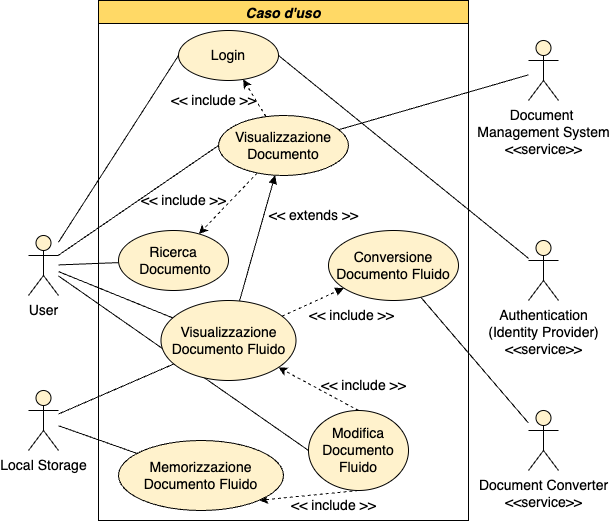
\includegraphics[width=1\textwidth]{img/tesi-1-Use-case.drawio.png}
\caption{Diagramma dei casi d'uso: funzioni/servizi offerti dal sistema Ebook App PoC}
\end{figure}

\begin{figure}[H]
\centering
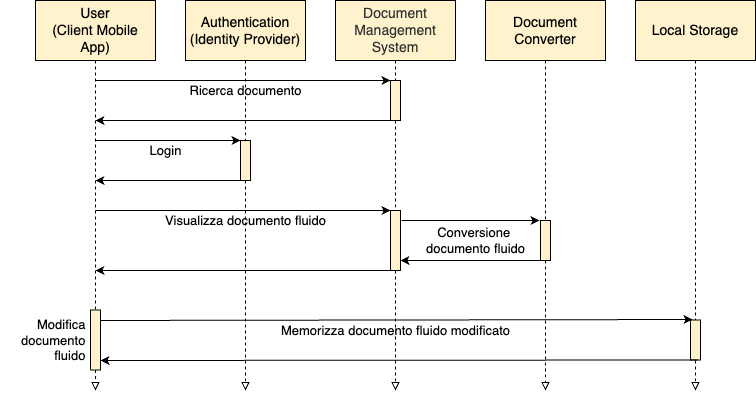
\includegraphics[width=1\textwidth]{img/tesi-2-Use-case2.drawio.png}
\caption{Diagramma di sequenza: scenario di modifica di un nuovo documento "fluido"}
\end{figure}


\section{Analisi Formati Digitali Fluidi}
I documenti attualmente sono reperibili in formato PDF e/o HTML. Il formato PDF è quello con cui i documenti vengono effettivamente archiviati: per ottenere un documento in formato HTML è necessario utilizzare un servizio interno, chiamato \textit{pdf2html}, il quale effettua la conversione. Entrambi i formati rispettano i requisiti per i documenti definiti "statici" ma non per quelli definiti "fluidi":
\begin{itemize}
    \item \textbf{PDF} (Portable Document Format) - Formato di file sviluppato da Adobe per rappresentare documenti di testo e immagini in modo indipendente dall'hardware e dal software utilizzati per generarli o per visualizzarli. Viene dunque generato e visualizzato con uno specifico layout.
    \item \textbf{HTML} (HyperText Markup Language) - Linguaggio di formattazione che descrive le modalità di impaginazione o visualizzazione grafica (layout) del contenuto, testuale e non, di una pagina web attraverso tag di formattazione. Viene generato tramite conversione del documento PDF riportando fedelmente il layout iniziale.
\end{itemize}
Per soddisfare i requisiti \textit{R1.1}, \textit{R2.1}, \textit{R5} e \textit{R6.1} il formato "fluido" deve:
\begin{itemize}
    \item rappresentare solamente il contenuto dei documenti "statici", rimuovendo tutte le formattazioni di layout,
    \item essere modificabile,
    \item poter essere ricavato convertendo un documento attualmente in formato "statico" (ovvero deve esistere un algoritmo/software per poter effettuare la conversione).
\end{itemize}
I formati attualmente disponibili che soddisfano i requisiti sopra indicati rappresentano implementazioni dello standard Open eBook (OeB), elaborato dall'Open E-book Forum. Tra questi i formati più diffusi sono:
\begin{itemize}
    \item \textbf{MOBI} (Mobipocket) - Standard proprietario (\textit{Amazon}) per la pubblicazione di libri digitali (eBook).\\
    Principali caratteristiche:
    \begin{itemize}
        \item basato sulla Open eBook standard utilizzando XHTML,
        \item annotazioni (highlights, segnalibri, correzioni, note e disegni) possono essere applicati, organizzati, e richiamati,
        \item può includere anche JavaScript e cornici.
    \end{itemize}
    \item \textbf{EPUB} (Electronic Publication) - Standard aperto specifico per la pubblicazione di libri digitali (eBook).\\
    Principali caratteristiche:
    \begin{itemize}
        \item basato sulla Open eBook standard utilizzando XML,
        \item a partire da settembre 2007 è lo standard ufficiale dell'International Digital Publishing Forum (IDPF)\footnote{\url{https://web.archive.org/web/20080827131750/http://www.idpf.org/2007/ops/OPS_2.0_final_spec.html}},
        \item CSS per il layout e la formattazione,
        \item testo "re-flowable" con grafica raster e vettoriale,
        \item disponibilità di diversi software, sia proprietari che open source, per la manipolazione del file (\textit{Adobe InDesign}, \textit{Sigil}, \textit{Calibre}, ...),
        \item disponibilità di tante librerie in diversi linguaggi per la manipolazione del file.
    \end{itemize}
\end{itemize}
Le caratteristiche determinanti che hanno portato alla scelta del formato EPUB sono state (\textit{i}) lo standard aperto e (\textit{ii}) la disponibilità, sia di software che di librerie, per la manipolazione del file. 

\section{Progettazione}
% Descrivere qua progettazione domini, boundaries, ecc secondo il DDD 
Nel redazionale non esistono i concetti di progresso di lettura, highlight, bookmark, appunto, ... -> modellato dominio in modo da gestire queste informazioni localmente senza modificare il dominio redazionale

\subsection{Ricerca Librerie}
Definiti i requisiti e modellato il dominio sono state individuate le seguenti librerie, suddivise per modulo, a supporto dello sviluppo della applicazione:
\begin{itemize}
    \item \textit{Shared}
    \begin{itemize}
        \item \textit{Ktor} - Framework asincrono per lo sviluppo di microservizi e applicazioni web. Nel progetto Ktor è utilizzato per la parte di networking come client HTTP.
        \item \textit{Kotlinx-Serialization} - Libreria multiplatform per la serializzazione dei dati.
        \item \textit{Kotlinx-Datetime} - Libreria multiplatform per la gestione delle date e del tempo.
        \item \textit{Kvault}\footnote{\url{https://github.com/Liftric/KVault}} - Libreria multiplatform per la persistenza dei dati sicura in formato chiave-valore. Tramite una unica API si comporta come wrapper di Keychain, nel caso iOS, e SharedPreferences nel caso Android.
        \item \textit{Koin}\footnote{\url{https://github.com/InsertKoinIO/koin}} - Dependency Injection framework multiplatform.
        \item \textit{Napier}\footnote{\url{https://github.com/AAkira/Napier}} - Logging framework multiplatform.
    \end{itemize}
    \item \textit{Android}
    \begin{itemize}
    \item \textit{Readium} (Kotlin-toolkit)\footnote{\url{https://github.com/readium/kotlin-toolkit}} - Libreria per la manipolazione e visualizzazione di contenuti editoriali digitali. Implementazione specifica per la piattaforma Android. 
    \end{itemize}
    \item \textit{iOS}
    \begin{itemize}
    \item \textit{Readium} (Swift-toolkit)\footnote{\url{https://github.com/readium/swift-toolkit}} - Libreria per la manipolazione e visualizzazione di contenuti editoriali digitali. Implementazione specifica per la piattaforma iOS. 
    \item \textit{KMPNativeCoroutines}\footnote{\url{https://github.com/rickclephas/KMP-NativeCoroutines}} - Libreria che permette l'utilizzo delle coroutine Kotlin in Swift in applicazioni Kotlin Multiplatform.
    \end{itemize}
\end{itemize}

\subsection{Readium}
Tra le librerie individuate quella fondamentale per il dominio applicativo è \textit{Readium}.
La necessità di un tool open-source, robusto e performante per la manipolazione e la lettura di formati editoriali digitali è alla base del progetto Readium. Essa infatti consiste in un insieme di toolkit per diversi formati (come epub, audiolibri e libri image-based) e diverse piattaforme (Android, iOS, Desktop e Web).\\
Readium è composto da quattro moduli principali:
\begin{itemize}
    \item \textit{Publication Server} - Fornisce le pubblicazioni tramite un server locale HTTPS.
    \item \textit{Streamer} - Modulo composto dai seguenti due sottomoduli:
    \begin{itemize}
        \item \textit{Parser} - Responsabile del parsing delle pubblicazioni e della loro esposizione utilizzando un modello in-memory.
        \item \textit{Fetcher} - Si occupa di ottenere i contenuti delle pubblicazioni e della loro manipolazione (in particolare injection di CSS e Javascript nelle risorse HTML).
    \end{itemize}
    \item \textit{Navigator} - Utile alla navigazione delle risorse di una pubblicazione secondo diverse strategie basate sulla natura della pubblicazione (ebook, audiolibri, ...). Interagisce con il modulo \textit{Streamer} per utilizzare il modello in-memory o per ottenere manifesto JSON attraverso il modello condiviso (\textit{Shared}).
\end{itemize}
\begin{figure}[H]
\centering
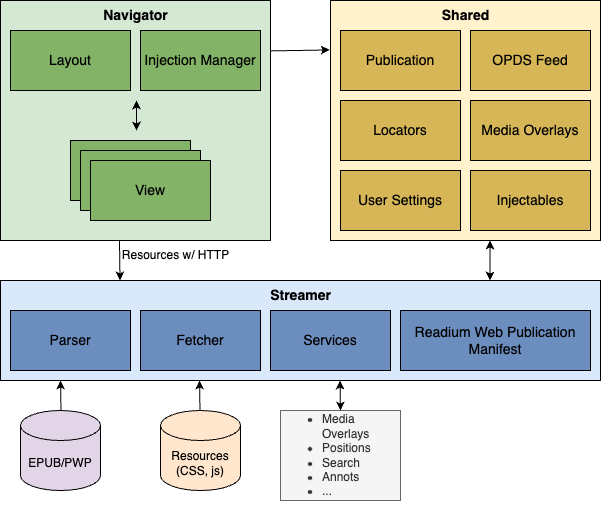
\includegraphics[width=1\textwidth]{img/tesi-22-readiumarch.drawio.png}
\caption{Architettura libreria Readium}
\end{figure}

\subsection{Architettura}
repository, dati remoti dal reda e dati locali per i preferiti, highlights ecc.

\subsection{Progettazione UI}
\begin{figure}[H]
\centering
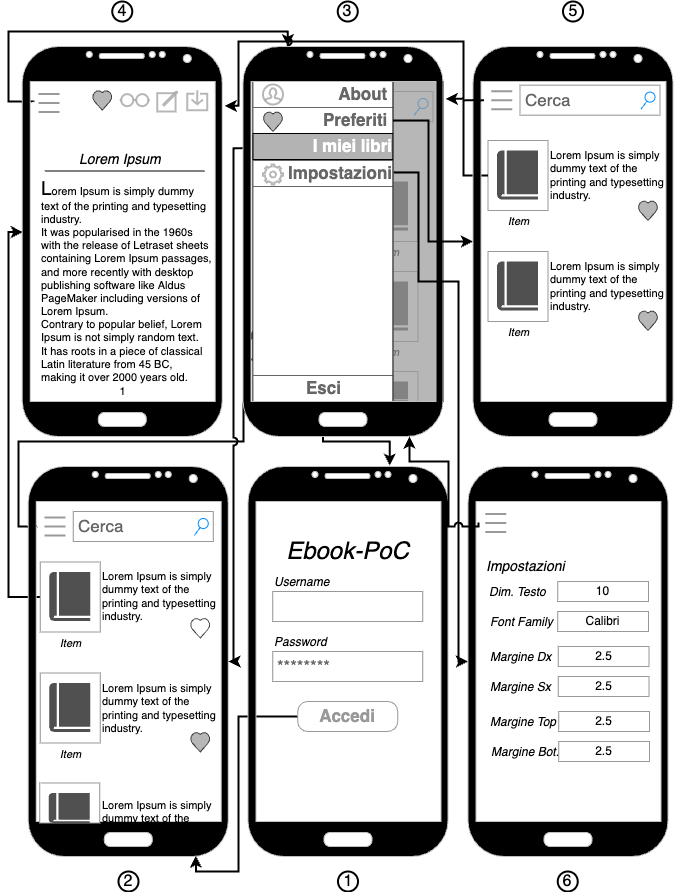
\includegraphics[width=1\textwidth]{img/tesi-14-mockup1.drawio.png}
\caption{Alcuni dei mockup realizzati per la progettazione e la validazione della UI (v1)}
\end{figure}

\section{Implementazione}

NavigationController e navigation graph per gestire il flusso tra i vari fragment della app. La fragment home è quella principale e prima di essere creata, se l'utente non ha fatto login, viene rediretto\footnote{\url{https://developer.android.com/guide/navigation/navigation-conditional}} al fragment di login per farlo autenticare e poi riportato indietro alla schermata di home (popStackBack)
\footnote{\url{https://medium.com/swlh/android-navigation-component-part-1-6191323eaf39}}.

Utilizzo di PagingData (Paging 3) per scaricare on demand il contenuto e mostrarlo nel recycler view con lo scroll.